\section{Методы анализа сортировок за квадратное время}
\epigraph{Если мы скажем, что проходим на лекции бабл сорт, то нас засмеют, поэтому назовем нашу лекцию так.}
{Г.О. Евстропов}

В процессе анализа алгоритма мы будем доказывать \textit{корректность} алгоритма и анализировать \textit{время его работы}. \par

Существуют хотя бы три метода доказательства корректности алгоритма (нам их должно хватить):
\begin{enumerate}
    \item по индукции;
    \item от противного;
    \item поиск инварианта.
\end{enumerate}

\begin{definition}
    «Задача о сортировке». Есть $n$ произвольных элементов $a_1, \ldots, a_n$. Хочется их упорядочить так, чтобы $a_{\pi(1)} \leq a_{\pi(2)} \leq \ldots \leq a_{\pi(n)}$.
\end{definition}

\textbox{
    \medskip
    \textbf{\large Лирическое отступление: RAM-модель} \par
    В нашей RAM-подели будет:
    \begin{itemize}
        \item 
            \begin{tikzpicture}
                \draw (0, 0) rectangle (0.3, 0.3);
            \end{tikzpicture}
            -- процессор. За единицу времени он умеет выполнять одно действие с целочисленными данными, а также запрос к одной ячейке пямяти.

        \item 
            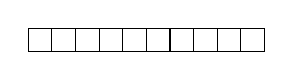
\begin{tikzpicture}
                \draw [step=0.3cm] (0, 0) grid (3, 0.3);
            \end{tikzpicture}
            -- память. Её всегда ассимпотически достаточно для любых действий (но не слишком много). Например, при $P(n)$ действий памяти будет примерно $c \cdot P(n)$. Кроме того, любая работа с куском памяти выполняется не быстрее, чем за длину этого куса.
    \end{itemize}

    Что мы умеем хранить и делать в RAM-модели:
    \begin{itemize}
        \item целые числа;
        \item вещественные числа;
        \item $\pm, \ *, /, \%$ за $O(1)$;
        \item все битовые операции выполняются за $O(1)$;
        \item всякие $\sqrt{x}, \sin{x}, \cos{x}, \ldots$ мы тоже умеем вычислять за $O(1)$ (если противное не оговорено заранее).
    \end{itemize}

}